% -*- TeX-PDF-mode: t; coding: utf-8; -*-
\documentclass[12pt,twoside,a4paper]{article}
\setlength{\oddsidemargin}{-0.4mm} % 25 mm left margin
\setlength{\evensidemargin}{\oddsidemargin}
\setlength{\textwidth}{160mm}      % 25 mm right margin
\setlength{\topmargin}{-5.4mm}     % 20 mm top margin
\setlength{\headheight}{5mm}
\setlength{\headsep}{5mm}
\setlength{\footskip}{10mm}
\setlength{\textheight}{237mm}     % 20 mm bottom margin

\usepackage[utf8]{inputenc}
%\usepackage{aeguill,mathptmx}  %% dummy package to make good PDFs

\usepackage{fontspec}
\setmonofont{PT Mono}
%\setmonofont{Menlo}

\usepackage[english]{babel}

\usepackage{hyphenat}
\usepackage{url}

% \usepackage{multicol}
% \usepackage{latexsym}
% \usepackage{longtable}
% \usepackage{alltt}

\usepackage{graphicx}
\usepackage[svgnames]{xcolor}

\usepackage{tikz}
\usepackage{pgfpages}
\usetikzlibrary{snakes}
% \usepackage{textcomp} 
% \usepgflibrary{arrows} % LATEX and plain TEX and pure pgf 
% \usetikzlibrary{arrows} % LATEX and plain TEX when using Tik Z 
% \usetikzlibrary{automata}
% \usepackage{pgf}

\usepackage[pdfauthor={Philippe Wang},%
colorlinks=true,urlcolor=black,%
linkcolor=black,citecolor=black,pdfpagelabels=false,pdfborder={0 0 0}%
]{hyperref}

\usepackage{listings}

\def\C{
  \lstset{
    basicstyle=\small\color{black}\ttfamily\small,
    inputencoding=latin1,
    upquote=false,
    language=C,
    keywordstyle=\color{black}\bfseries, 
    identifierstyle=, % nothing happens
    commentstyle=\color{black!70!white},
    stringstyle=\ttfamily,
    showstringspaces=true,
    numberstyle=\tiny\em,
    backgroundcolor=\color{white!90!blue},
  }
}

\def\OCaml{
  \lstset{
    basicstyle=\small\color{black}\ttfamily\small,
    inputencoding=latin1,
    upquote=false,
    language=[Objective]caml,
    keywordstyle=\color{black}\bfseries, 
    identifierstyle=, % nothing happens 
    commentstyle=\color{black!70!white},
    stringstyle=\ttfamily,
    deletekeywords={ref,or},
    showstringspaces=true,
    numberstyle=\tiny\em,
  }
}
\C

\author{Philippe  Wang}

\title{Illuminate: managing microcontrollers for comfortable
  energy-efficient LED-based lighting}

\date{}


\def\eg{\emph{e.g.}}
\def\ie{\emph{i.e.}}
\def\RPI{Raspberry-$\pi$}
\long\def\todo#1{{\color{red}TODO #1}}

\begin{document}
% \setcounter{page}{3}

\maketitle

\begin{abstract}
  A  network of  hundreds (or  more) of  LED-and-ARM-m0-based lighting
  devices  raises  many  programming  constraints due  to  the  little
  capacities   offered    by   the   very    energy-efficient   ARM-M0
  microcontrollers, the  measurements we want to make  and the actions
  we  want to  take,  and of  course  the management  of that  network
  itself. This paper presents  those constraints and proposes a simple
  programming model to address them.
\end{abstract}


%%%%%%%%%%%%%%%%%%%%%%%%%%%%%%%%%%%%%%%%%%%%%%%%%%%%%%%%%%%%%%%%%%%%%%
\section{Introduction}

An LED (Light-Emitting Diode)  is a semiconductor electronic component
that emits light  when traversed by an electric  current.  In the past
decade, high-power  LEDs have made significant progress  in the market
of   lighting  devices  while   they  are   becoming  more   and  more
energy-efficient. LEDs capable of  emitting more than a hundred lumens
(lm) per watt (W) are no  longer the exception. We may compare that to
the 16 lm/W of a typical incandescent  light bulb or to the 60 lm/W of
a  compact fluorescent  light bulb,  which make  LEDs  interesting for
saving energy.   LEDs also  advertise a very  long lifetime (10  to 30
years),  which make  them interesting  for reducing  maintenance work.
And  as LEDs  are  electronic  components, it  only  seems natural  to
accompany them with sensors and other electronic components.  Then, to
manage those multiple components, the  use of a microcontroller is the
obvious solution if we want to keep the possibility to reprogram them
at will.

Today, microcontrollers  are tiny  computers that consume  very little
energy and  are widely spread  in industry robots,  electronic devices
and    home     electric    appliances.     An     ARM    Cortex    M0
microcontroller\cite{m0web,m0tech} has a computing power comparable to
an IBM PC or an Apple Macintosh from the 1980s.

In this project we consider  the ARM Cortex M0 microcontroller family,
which groups 32-bit ARM  V6-M chips. They have a few kB  of RAM, a few
tens  kB of  flash memory  and they  run  at a  few tens  of MHz.   So
basically their microprocessors run faster than those of 1980s PCs but
they have less RAM.

In order to ease the programming of those chips, we use the LPCXpresso
LPC1115 platform,  which are shipped with  8kB of RAM, 64  kB of flash
memory and a 50 MHz  ARM V6-M processor which handles 56 instructions.
Those  have  the advantage  of  providing  a ready-to-use  programming
environment (\ie, an Eclipse-based IDE and some convenient libraries).
There  are  platforms  that  can  be  software  compatible  and  which
performance differ more or less (\eg, the LPC1114 precedes the LPC1115
and   essentially   provides  half   the   flash   memory  and   fewer
registers\cite{LPC111X,UM10398}) and  there might  be new ones  in the
future, and we may switch to one of them if need be.

This paper is organized as follows.
Section \ref{sec:HLR} lists our high-level requirements.
Section \ref{sec:hardware} lists hardware properties that are important
to be aware of for this project.
Section \ref{sec:programming-model} sums up the software constraints
and proposes a programming model for our network of light devices.
Section \ref{sec:conclusion} concludes our paper.

\section{High-level requirements}
\label{sec:HLR}

This section lists the main high-level requirements.

\begin{itemize}
\item The devices provide enough light.
\item The devices should not enter an annoying state that would
  disturb the working environment (\eg, blinking when no hazard or
  changing the light intensity or color for no valid reason).
\item The devices should be reprogrammable if we need to deploy new
  software implementation.
\item The devices should function in case of emergency (\eg, fire).
\item The devices should help detect fire and alert the relevant
  authorities in case of hazard.
\item The devices should detect important hardware anomalies.
\item The light temperature should adjust according to outdoor light
  (warm light to cold light to warm light).
\item The lights should be in an energy-saving mode when there's no
  human presence.
\item Use low-level unsafe languages as little as possible.
\item Overall, the system should be reliable.
\end{itemize}

\section{Hardware considerations}
\label{sec:hardware}

\subsection{Overview}

Figure \ref{fig:subnetwork} shows a scheme of what we have in mind.

\begin{figure}[bth]
  \centering
\framebox{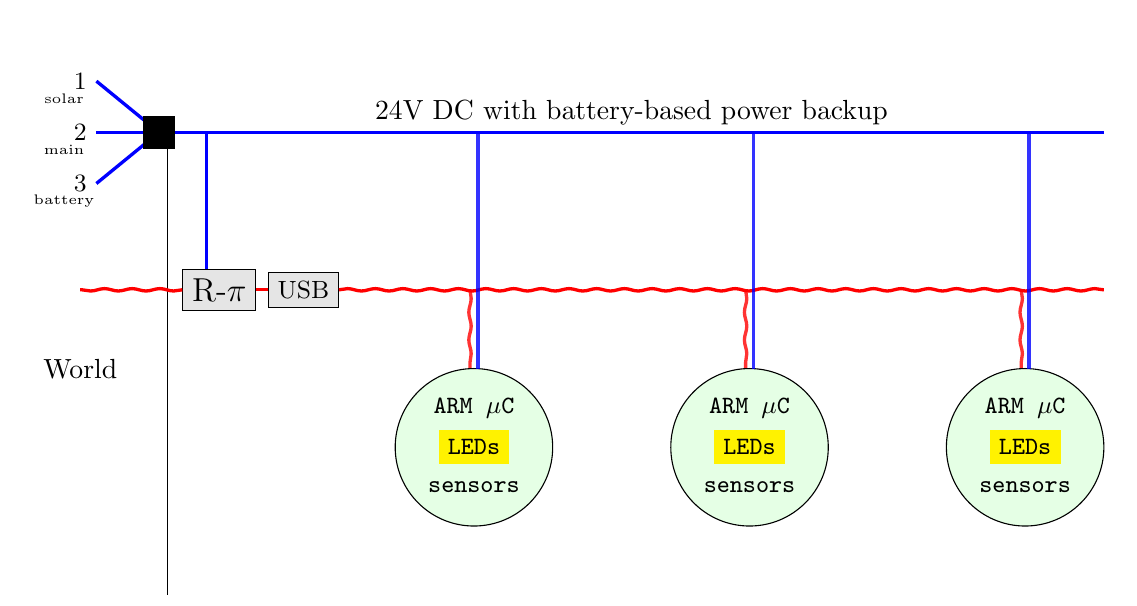
\begin{tikzpicture}[fill=yellow]
  \def\eow{12}
  \node at (6,0.25) {24V DC with battery-based power backup};
  \node (24) at (0.23,0) {};
  \node (o24) at (0.23,-6) {};
  \draw (24.north west) -- (o24.north west);
  \draw [blue, very thick] (0,0) -- (\eow,0);
  % \draw [red, very thick] (0,-0.1) -- (\eow,-0.1);
  \node (b) at (1.3,-2) [] {~~~~~~~~};
  \draw[blue,very thick] (0.6,0) -- (0.6,-2);
  % \draw[red,very thick] (0.7,-0.1) -- (0.7,-2);
  \node (rpi) at (b.west)  [draw,fill=white!90!black] {\large R-$\pi$};
  \node (usbe) at (b.east)  [draw,fill=white!90!black] {\small USB};
  \draw[red,very thick,snake=snake,segment amplitude=0.1ex,segment length=1em]
       (rpi.west) -- (-1,-2);
  \draw[red,very thick,snake=snake,segment amplitude=0.1ex,segment length=1em]
       (rpi.east) -- (usbe.west);
  \draw[red,very thick,snake=snake,segment amplitude=0.1ex,segment length=1em]
       (usbe.east) -- (\eow,-2) ;
% \node at (6,-1.7) {communication};
  \def\sep{3.5}
  \foreach \x in {0,1,2} {
    \draw[red,very thick,snake=snake,segment amplitude=0.1ex,segment length=1em,opacity=0.8]
         (4+\sep*\x-0.05, -2) -- (4+\sep*\x-0.05, -3);
    \draw[fill=green!10!white] (4+\sep*\x, -4) circle (1);
    \node at (4+\sep*\x, -3.5) [] {\tt\small ARM $\mu$C};
    \node at (4+\sep*\x, -4) [fill=yellow] {\tt\small LEDs};
    \node at (4+\sep*\x, -4.5) [] {\tt\small sensors};
    \draw[blue,very thick,opacity=0.8]
         (4+\sep*\x+.05, -3) -- (4+\sep*\x+.05, 0);
  }
  \node at (-1,-3) {World};
  \node (1) at (-1,0.65) {\small 1};
  \node (2) at (-1,0) {\small 2};
  \node (3) at (-1,-0.65) {\small 3};
  \node at (1.south west) {\tiny solar};
  \node at (2.south west) {\tiny main};
  \node at (3.south west) {\tiny battery};
  \foreach \x in {1,2,3} {
    \draw [blue,very thick] (\x.east) -- (0,0);
    % \draw [red,very thick] (\x.base east) -- (0,-0.1);
  }
  \draw[fill=black] (-0.2,-0.2) rectangle (0.2,0.2) ;
\end{tikzpicture}}
  \caption{subnetwork}
  \label{fig:subnetwork}
\end{figure}


\paragraph{Three sources of electric power.} Whenever available, we
use solar  energy. If they fail,  notably when the  sun is unavailable
because of weather conditions or simply because it's night, we use the
main power.  If the main power  goes down, we rely  on batteries. That
way we shall always be able  to light the building even in exceptional
cases. 

\paragraph{Reusing  the  existing electric  wiring}  avoids having  to
redeploy wires through our  entire infrastructure. And to avoid having
to  convert  alternating current  to  direct  current  many times,  we
provide a main  24V direct current.  As the wires  are not twisted nor
shielded, they  might cause or be victim  of electrical interferences.
\textit{Note that using  an existing wiring designed for  at most $n$W
  at 240V means that at 24V  we should allow at most $(n/10)$W in
  those wires.}

\paragraph{A hierarchy of devices.} A  set of lighting devices will be
controlled by a larger  computer, probably a Raspberry-$\pi$, which is
basically a small computer characterized by an ARM processor at 700MHz
with 512 MB  of RAM, an SD  card reader, a 10/100 Ethernet  port and 2
USB2 ports. The \RPI{}s will  notably be the relay between the outside
world and the lighting devices.

\paragraph{Communication} will  be assured by an  implementation of an
Ethernet-like protocol. A USB device  will be plugged to the \RPI{} to
assure the communication with the multiple lighting devices.

\paragraph{Board  design.}   Each   lighting  device  carries  an  ARM
microcontroller,  a set  of  LEDs and  a  set of  sensors. For  safety
purposes,  the   sensors  and  the   LEDs  will  be  accessed   via  a
co-microcontroller (another  tinier ARM chip) which  sole purpose will
be to abstract the very low-level computations for probing the sensors
or setting the current intensity for the LEDs.

\subsection{LEDs}

\paragraph{Light intensity}

There are  two ways  for controlling the  light intensity for  an LED.
Either  we change  the current  that  powers the  LED, or  we use  the
pulse-width modulation technique, which basically consists of powering
the LED  for a fraction  of second, then  not powering it  for another
fraction  of second,  and go  on this  way.  Contrary  to incandescent
light bulbs, when an LED  stops being powered, it stops emitting light
very quickly (almost immediately), so the blinking has to be very fast
for the human eyes not to be  able to notice it.  We may consider that
the human  eyes cannot notice  that an LED  is off when it  lasts less
than a 1/100 second.   To power an LED at 10\%, we  may have it on for
1/1000  second  and  off for  9/1000  second.  Note  that due  to  the
persistence of  vision phenomenon, we  might perceive it as  more than
10\%.

There are two ways to  implement the pulse-width modulation technique:
either  the  microcontroller  commands  a  transistor  at  the  wanted
frequency and the state of the  transistor will match the state of the
LED,  or it  delegates the  task to  another device.

To  implement  the  current  variation,  we can't  rely  just  on  the
microcontrollers because they don't  actually provide the current that
actually powers  the LEDs since that  current would be quite  too high
for them to handle, so it relies on an external device.

In  practice, changing  the  current  for an  LED  means changing  the
voltage but  it is  important to  note that as  for other  diodes, the
current  is exponentially dependent  on the  voltage according  to the
\emph{Shockley     ideal     diode     equation}    or     \emph{diode
  law}\cite{Shockley-diode-equation}.
% http://en.wikipedia.org/wiki/Diode#Shockley_diode_equation
This means that we must be able to control the voltage very precisely.
Note that  for incandescent  light bulbs, it  is very  different since
light output  and power consumption are  approximately proportional to
the voltage.


\paragraph{Colour temperature}

There are different white lights, which go from a warm yellowish white
(2700K)  to  a cold  blueish  white  (6400K).  Basically,  the  former
corresponds to sunrise  and sunset lights as the  sunlight is filtered
by a large part of the Earth's atmosphere, and the latter, also called
daylight,  corresponds  to the  sunlight  when  it's the  most  direct
(zenith) and little filtered by the atmosphere.

Matching  the colour  of interior  light with  the colour  of sunlight
allows more  comfort. This can be  achieved by using  a combination of
LEDs, which  could be a  set of  RGB LEDs or  a set of  warm-light and
cold-light LEDs.

By varying the intensities of each  LED of a warm-light and cold-light
LEDs set, we may obtain the colour temperature that corresponds to the
outdoor light.

The outdoor  light can  simply be  approximated by  the date  and time
information, or  can be more  precise if  measured by sensors,  as the
outdoor light also depends on the presence and thickness of the clouds
that are traversed by the  sunlight.  However placing the sensors that
are required for this measurement might demand too much effort.

\paragraph{LED aging}

Contrary to incandescent light bulbs, which are basically a thin metal
filament  that emits light  when traversed  by some  electric current,
LEDs “natural death” is not sudden. Indeed, LEDs light intensity slowly
diminishes over time, so at  some point they shall be replaced because
they do not  fill their duties anymore even if  they still emit light.
This also  means that if  at the start  we use LEDs that  are brighter
than  necessary, we  should obtain  an overall  longer  lifespan.  The
maximum intensity will  only be required when the  LEDs have lost some
light  intensity potential, and  after that  time, they  will continue
losing light intensity until they should be replaced.

However, an  LED-based lighting device lifespan also  depends on other
electronic  components.  So, which  ever irreplaceable  component dies
first  will take the  rest with  it, which  means that  short lifespan
components should be made easy to replace.

Deploying thousands of devices will certainly give interesting data
on that matter.


\subsection{Sensors}

\subsubsection{Temperatures}

\paragraph{Room  temperature} may be  measured with  thermometers that
should  be deported  because  it's  quite likely  that  the LEDs  will
generate too  much heat  for the temperature  to be accurate  near the
LEDs.   This   information  may  allow  to   analyse  the  temperature
variations over a long period of  time (days, weeks or months) or more
precise information over  a shorter period of time  (hours, minutes or
seconds).

\paragraph{Hardware temperatures} may  allow to detect overheating and
adjust the power that is provided to the LEDs. We may use such data to
analyse  the evolution of  the temperature  according to  other inputs
(\eg, room temperature, light-on duration, air flow)

\subsubsection{Light}

Ambient light information may help determine if LEDs are still working
properly or determine  if it's necessary to switch  the LEDs on.  Such
sensors would give different  information depending on where they are:
close to  the LEDs, they loose  information when the LEDs  are on, and
far from the LEDs, they are quite less easy to deploy.

\subsubsection{Infrared}

Heat  detection for  movement and  people detection.   Direct sunlight
might  alter the relevance  of infrared  sensor information,  but that
depends on if it's  a simple cell or a set of  cells and in the latter
case, it depends on how they perceive information: blurry or a sharp
picture which would allow shape recognition.

\subsubsection{Sound}

It would be interesting to measure  the ambient noise, and this could be
used to help people find a quite place.

\subsubsection{CO$_2$}

The concentration  of carbon  dioxide in the  air may allow  to detect
fire as the former increases rapidly when the latter occurs.

\subsection{ARM M-0 microcontrollers}

\subsubsection{GPIOs}

LPC1115 have 42 general purpose input/output pins that operate at 1.8V
to 3.6V.  Each of  them can output up to 20 mA  of current and this is
considered high. The maximum power output is then 72 mW,
so it's  quite impossible  to  directly provide  the current  for
powerful LEDs  from a LPC1115.

GPIOs will be used to drive LEDs but also for communication.


\subsubsection{Input and output operations}

% How to set a bit field

The following  C code snippets show  how a pin  can be set to  let the
current   pass   (function   \texttt{on})   or  not   pass   (function
\texttt{off}).

\C
\begin{lstlisting}
void on() {
	LPC_GPIO0->DATA |= 1<<7;
}
\end{lstlisting}
\begin{lstlisting}
void off() {
	LPC_GPIO0->DATA &= ~(1<<7);
}
\end{lstlisting}


Most   microcontrollers  are   programmed  using   unsafe  programming
languages. They are unsafe in  the sense that they don't automatically
detect some operations that can't be right, like writing on a pin that
we want read-only,  or more generally write or read  memory at a wrong
location. Of  course, no language automatically  detects every mistake
that the programmer makes.  However there exist languages which design
help  detecting a large  part of  most common  errors.  A  strong type
system is a good base for that purpose.


\subsection{The notion of time}

There many ways to represent and see time:
\begin{enumerate}
\item  the  continuous  time   that  goes  by  and  virtually  affects
  everything the same way, we use atomic clocks as references;
\item the  discrete time from an ARM  chip point of view,  that is the
  ticks given by one or several (generally quartz) clocks;
\item  an abstract  and  discrete notion  of  time as  in the  Esterel
  programming   language\cite{Esterel1992,Esterel1999},   where   each
  instant is  separate from other  instants, and each instant  or tick
  may last a variable amount of real continuous time.
\end{enumerate}
And those times often run at different speeds, and if we need them to
run at virtually the same speed, we need to synchronise them.

In  programming, we  can't really  deal with  continuous  time because
there's  a mathematical barrier  that prevents  a computer  from being
able to really represent real numbers. Therefore, we use discrete time
and  often pretend  that it's  “continuous” because  it's then  a good
approximation indeed.

Reasoning about programs  on hardware clocks is not  too hard with ARM
microcontrollers because  there are not  any page faults,  each atomic
operation  on the  processor should  always  take the  same amount  of
discrete time (\ie,  the same amount of cycles).  Then if we introduce
real time constraints because we have human users, it becomes somewhat
harder since we need to synchronise the hardware clock with real time.
It  easily  becomes  quite  difficult  if we  don't  have  homogeneous
hardware clocks  (\eg, one device has  a 50 MHz  processor and another
has a 40 MHz  one). However if we know the lower  bound, we can always
synchronise the  programs on different  hardware by inserting  NOPs in
the programs for the faster processor(s).

Esterel's model of  time is quite convenient when  we have events that
happen  at  the “same  time”,  or  should we  say  here  “at the  same
instant”, and  we struggle with programming the  handlers because they
easily  get  stuck  on   race  conditions.   However  Esterel  doesn't
guarantee anything  on the  amount of real  time that an  instant will
take. The obvious practical reason  for that is that Esterel allows to
generate program  skeletons that completely deal  with the concurrency
issues  but those  skeletons  are filled  by  some programmers  (which
generally  are human)  with  things  that may  offer  no guarantee  on
execution time.

\section{Standard environment to programming LPC platforms}

\todo{.}

\section{Programming model}
\label{sec:programming-model}

There are actually only quite a limited number of primitive operations
that we  want to run on  a lighting device. We  want it to  be able to
communicate  its  state,  receive   orders  (\eg,  setting  the  light
intensity),  and operate a  few things  on its  own (\eg,  varying the
light intensity on its own to  alert people of a danger). Therefore it
seems  relevant  to  provide  a  small  abstract  machine  because  it
simplifies the  programming model  and allows us  to reason  about it,
which provides us with more confidence.

However, as the ARM M0 we use has only a very limited amount of RAM (8
kB),  which   will  already  be  partly  used   for  implementing  the
communication  protocols (lower-level  and  higher-level), it  doesn't
seem  like a  good  idea to  implement  an abstract  machine that  may
automatically allocate a  lot of memory. Still, if  it does, it should
be either for some data that  rarely changes so that it can be written
on the flash memory without  wrecking it prematurely (\eg, it may seem
relevant to  allocate some data  that will basically not  change until
the  next  major  update  or   reboot),  or  some  data  that  can  be
garbage-collected  quickly enough  to avoid  any failure  to allocate.
Although, it  is still unclear  that being able  to allocate a  lot of
short-lifetime objects would  be an actual asset, as  such objects are
typically closures or other functional data structures.

Allowing explicit  memory allocation and deallocation  on the abstract
machine  side would  mean  to expose  vulnerabilities.  It seems  more
appropriate to limit such operations.


\subsection{A   language  to   program  the   lighting   devices  with
  asynchronous watchers}

In this section, we present a small language that should be enough and
convenient to program our lighting devices.  The main particularity of
this language is that it provides asynchronous tasks registration, and
that fits quite well with what we expect from the lighting devices.


Here follows an OCaml representation of the language.

\OCaml
\begin{lstlisting}
type command =
| Reset
| Named of id * commands     (* procedure     *)
| Call of id                 (* invoke        *)
| Repeat of int * commands   (* bounded loop  *)
| Run_at of time * commands  (* absolute time *)
| Run_in of time * commands  (* relative time *)
| Set_intensity of id * int
| Get_intensity of id        (* communication *)
| Alert of id * int          (* communication *)
| Set_time of time
| Get_time of time
| On_out_of_abs_range of id * l_bound * u_bound * commands * validity
| On_out_of_rel_range of id * l_bound * u_bound * commands * validity
| On_in_abs_range     of id * l_bound * u_bound * commands * validity
| On_in_rel_range     of id * l_bound * u_bound * commands * validity
| If of comparison * commands * commands
and comparison =
| GT of id * int
| GE of id * int
| EQ of id * int
| LT of id * int
| LE of id * int
and l_bound = int  (* lower bound *)
and u_bound = int  (* upper bound *)
and validity = int (* validity in number of VM cycles, with 0 for infinity *)
and commands = command list
and id = int
\end{lstlisting}
% - Time tasks could use an array-based queue to have good performance
% in space and time, but that implies that the time range is small enough.
% - A loop runs "cycles", at each cycle it performs a set of checks to
% do the tasks.

\subsubsection{Implementation on the lighting devices}

Each command may be represented by an element of a C
\texttt{enum}.

\C
\begin{lstlisting}
enum command {
  RESET,
  NAMED,
  CALL,
  REPEAT,
  RUN_AT,
  RUN_IN,
  SET_INTENSITY,
  GET_INTENSITY,
  ALERT,
  SET_TIME,
  GET_TIME,
  ON_OUT_OF_ABS_RANGE,
  ON_OUT_OF_REL_RANGE,
  ON_IN_ABS_RANGE,
  ON_IN_REL_RANGE,
  IF
};
\end{lstlisting}

The interpreter may be shaped as follows.
\begin{lstlisting}
void interp() {
  command** tasks = init_tasks();
  command** call_stack = (command**) malloc(CALL_STACK_SIZE);
  while(1) {
   asynchronous_tasks();
   switch(get_instr()) {
    case RESET: Reset(); break;
    case NAMED: Named(); break;
    case CALL:  Call(); break;
    case REPEAT: Repeat(); break;
    case RUN_AT: Run_at(); break;
    case RUN_IN: Run_in(); break;
    case SET_INTENSITY: Set_intensity(); break;
    case GET_INTENSITY: Get_intensity(); break;
    case ALERT: Alert(); break;
    case SET_TIME: Set_time(); break;
    case GET_TIME: Get_time(); break;
    case ON_OUT_OF_ABS_RANGE: On_out_of_abs_range(); break;
    case ON_OUT_OF_REL_RANGE: On_out_of_rel_range(); break;
    case ON_IN_ABS_RANGE: On_in_abs_range(); break;
    case ON_IN_REL_RANGE: On_in_rel_range(); break;
    case IF: If(); break;
    default: break;
   }
  }
}
\end{lstlisting}

The interpreter should use a few variables to represent 
some registers such as the program counter and the stack.

\begin{lstlisting}
#define asynchronous_tasks() do {            \
  push(call_stack, instr);                   \
  command* task;                             \
  while(task = pick_task(tasks)) run(task);  \
  instr = pop(call_stack);                   \
} while(0)
\end{lstlisting}

Abstractions over commands such as those to get data means giving more
responsibility to the compiler.

\begin{lstlisting}
// Getting the data
// All these functions are almost the same, they just get one or several
// bytes and return them. Multiple functions means more precise type
// checking.
// The data is either coming from the VM's memory (registered tasks)
// or the Master (R-pi).

/* get_instr() returns the next instruction to be executed */
command get_instr();

/* get_next_half_byte() returns the next half byte */
char get_next_half_byte();

/* get_next_byte() returns the next byte */
char get_next_byte();

/* get_next_2bytes() returns the next 2 bytes */
short get_next_2bytes();

/* get_next_2bytes() returns the next 4 bytes */
int get_next_word();
\end{lstlisting}

Write operations to  the flash memory should be  abstracted to improve
execution safety.

% How to reserve space in Flash:
% \url{http://www.support.code-red-tech.com/CodeRedWiki/ReserveFlash}
\begin{lstlisting}
// Write data in the flash memory
void* write_data(int size, command* cmds);
\end{lstlisting}



\section{Conclusion}
\label{sec:conclusion}

\todo{.}

\def\URL#1{{\\\footnotesize\url{#1}}}
\bibliographystyle{plain}
\bibliography{references}

\todo{.}

\tableofcontents

\end{document}

